\documentclass{scrreprt}
\usepackage{listings}
\usepackage{underscore}
\usepackage[bookmarks=true]{hyperref}
\usepackage[utf8]{inputenc}
\usepackage[french]{babel}
\usepackage{graphicx} %package pour ajouter les images
\usepackage{array} % pour les tableaux
\usepackage[nottoc, notlof, notlot]{tocbibind} %pour afficher la biblio ?
\usepackage{amsmath}
\usepackage{breqn}
\usepackage{multicol}
\hypersetup{
    bookmarks=false,    % show bookmarks bar?
    pdftitle={Software Requirement Specification},    % title
    pdfauthor={GUYO MARIE-JEANNE},                     % author
    pdfsubject={TeX and LaTeX},                        % subject of the document
    pdfkeywords={TeX, LaTeX, graphics, images}, % list of keywords
    colorlinks=true,       % false: boxed links; true: colored links
    linkcolor=blue,       % color of internal links
    citecolor=black,       % color of links to bibliography
    filecolor=black,        % color of file links
    urlcolor=purple,        % color of external links
    linktoc=page            % only page is linked
}%
\def\myversion{1.0}
\date{}
%\title

\usepackage{hyperref}
\begin{document}

\begin{flushright}
    \rule{16cm}{5pt}\vskip1cm
    \begin{bfseries}
        \Huge{Projet d'initiation à la découverte et à la recherche \\ PIDR}\\
        \vspace{1.9cm}
        \LARGE{Encadrant: Samuel MARTIN}\\
       \vspace{10.9cm}
	\begin{center}
		GUYO Albert\\
		MARIE-JEANNE Rémi\\
	\end{center}
        \vspace{1.9cm}
    \end{bfseries}
\end{flushright}

\tableofcontents
\newpage
\begin{multicols}{2}

\chapter{Étude des articles}

\section{Présentation des articles}

Les deux articles que nous allons étudier sont “Social influence networks and opinion change”, écrit par Noah E. Friedkin et Eugene C. Johnson \cite{FJ} et “Modelling influence and opinion evolution in online collective behaviour”, de Corentin Vande Kerckhove, Samuel Martin, Pascal Gend, Peter J. Rentfrow, Julien M. Hendrickx et Vincent D. Blondel \cite{VMG}.\\

L’article \cite{FJ} de Friedkin et Johnson porte sur les dynamiques d’opinion. C’est-à-dire la façon dont des individus peuvent modifier leurs opinions lorsqu’ils sont confrontés à un groupe de personne. Plus précisément, il s’interroge sur la possibilité de parvenir à un consensus entre les acteurs. Le document a été écrit en 1999. De nombreuses études avaient déjà été menées depuis 1950, notamment par John French, dont on peut citer l'article "A formal theory of social power" \cite{French} de 1956 ou encore Ash, à qui l'on doit "Effects of group pressure upon the modification and distortion of judgments" \cite{Asch}.\\

Le second article \cite{VMG}, plus récent, date de 2016. Il reprend le thème des dynamiques d’opinion mais avec une théorie différente de la précédente. L'article évalue la capacité d'un modèle simple à prédire l'évolution de l'opinion.

\section{La théorie présentée}

L’objectif de l'article \cite{FJ} est de parvenir à valider un modèle reliant l’évolution de l’opinion d’un individu en la confrontant à celle d’autres individus. Les participants pouvaient être encouragés, ou non, à parvenir à un consensus. Le modèle proposé relie l’opinion d’une personne $i$ à l’instant $t$ à l’opinion de tous les autres participants à l’instant $t$-1 ainsi qu’à son opinion initiale. On la note $y_i(t)$. On a :\\

\begin{equation}
\label{1}
y(t) =AWy(t-1)+(I-A)y(1), 
\end{equation}

avec $y(t)=(y_1(t), y_2(t), ... , y_n(t))^T$ le vecteur de taille $N$ contenant la valeur de l’opinion des $N$ participants à l’instant $t$, $A=diag((a_{ii})_i)$, la matrice diagonale de taille $N\times N$, où $a_{ii}$ représente le poids que l'individu $i$ accorde à l'opinion des autres participants, $W$ la matrice diagonale $N\times N$, avec $w_{ij}$ l’influence de l’individu $j$ sur l’individu $i$, avec $\sum_{i=1}^{N} w_{ij} = 1$. \\

 Il est possible de poser :\\
\begin{equation}
\label{WC}
 W=AC+I-A,
\end{equation}

où C correspond à la matrice $N \times N$ d'influence relative. Le poids $c_{ij}$ correspond à l'influence de j sur i. Tous les coefficients diagonaux de C sont nuls et $\sum_{i=1}^{N} c_{ij} = 1$. \\

Le modèle proposé dans l'article \cite{VMG} est similaire au précédent. Cependant, l’influence initiale n'intervient plus dans la formule.\\

\begin{equation}
\label{2}
y(t) =(I-A'(t-1))y(t-1)+A'(t-1)\bar{y}(t-1) 
\end{equation}

On remarque qu’ici, la matrice $A' = diag(a_{ii})$ qui représente l'influençabilité dépend de l’instant auquel on effectue l’expérience. En effet, au bout d'un certain nombre de répétitions, l'opinion de l'individu n'évolue plus. Il n'est donc plus affecté par l'opinion des autres et son influençabilité diminue. La variable $\bar{y}(t)$ représente la moyenne des valeurs des opinions à l’instant $t$. On peut aussi écrire la formule \eqref{2} sous la forme :

\begin{dmath}
\label{3}
y(t) = (I-A'(t-1))y(t-1) + A'(t-1)(\frac{1}{n} \textbf{1} ^T\times \textbf{1}) y(t-1).
\end{dmath}

En identifiant avec la formule \eqref{1}, on remarque que $W=(\frac{1}{n} \textbf{1} ^T\times \textbf{1})$. Ainsi, on donne le même poids à chaque autre individu.\\

Nous pouvons alors dresser un comparatif des deux modèles dans la Table 1.1.\\

\end{multicols}

\begin{table}
	\begin{tabular}{|p{3cm}|p{3.375cm}|p{3.375cm}|p{3.375cm}|}
		\hline
 & Friedkin et Johnson \cite{FJ} & Van de Kerckhove et al. \cite{VMG} & Interprétation \tabularnewline
		\hline
Coefficient devant l'opinion initiale & $I-A$ & $0$ & L'opinion initiale n'est pas prise en compte dans l'article \cite{VMG} \tabularnewline
		\hline
Coefficient devant la réponse de l'individu à l'instant précédent & $A(A-I)$ & $(I-A'(t-1))$ & Dans le modèle  \cite{VMG}, Le poids donné à sa propre opinion varie au bout du temps \tabularnewline
		\hline
Coefficient devant l'opinion du groupe à l'instant précédent & $A^{2}C$ & $A'(t-1)(\frac{1}{n} \textbf{1} ^T\times \textbf{1})$ & Dans l'article \cite{VMG}, la même influence est attribuée à chaque participant sur l'individu \tabularnewline
		\hline
	\end{tabular}
	\caption{Comparaison des 2 modèles}
\end{table}

\begin{multicols}{2}

\section{Expériences et méthode mises en oeuvre}


\subsection{Description de l'expérience}

Les deux articles étudiés présentent chacun une expérience cherchant à montrer la validité de leur modèle.\\

Dans l’article de Friedkin et Johnson \cite{FJ}, l’expérience consistait à former des groupes de deux à quatre personnes. Un total de 368 personnes a participé. Une question était posée à chaque groupe, par exemple : \textit{À combien estimez-vous le salaire horaire des travailleurs non-diplômés  travaillant sur un site de désamiantage ?}. Les individus donnaient chacun un résultat. S’ensuivait une conversation téléphonique avec d’autres participants. Ils pouvaient alors donner une nouvelle réponse. L’opération se répétait jusqu’à ce que la situation n’évolue plus et tous les résultats intermédiaires sont conservés. Il est ensuite demandé aux différents participants d’estimer à quel point ils pensent avoir été influencés par les autres. Pour ce faire, ils devaient répartir une pile de jetons de poker.\\

Dans le cas de l’article \cite{VMG}, une plateforme de crowdsourcing a été utilisée afin de recruter 861 sujets. Un groupe était formé de six personnes ou moins. Deux jeux leurs étaient proposés. Le premier consistait à évaluer le nombre de points dans une image. Le second à évaluer la proportion d'une couleur dans une image. Le jeu était divisé en trois phases. Par exemple, pour le premier jeu, lors de la première phase, l'individu devait évaluer, seul, le nombre de points présents sur chacune des 30 images. Lors de la seconde phase, il avait accès aux estimations des cinq autres participants, et pouvait modifier ses réponses en conséquence. La troisième phase correspond à une répétition de la deuxième phase. Les estimations alors présentées sont celles de la deuxième phase. \\

Bien que ces expériences présentent des similitudes, elles possèdent des différences notables résumées dans la Table 1.2.\\

\end{multicols}

\begin{table}
	\begin{tabular}{|p{4cm}|p{4.5cm}|p{4.5cm}|}
		\hline
 & Friedkin et Johnson \cite{FJ} & Vande Kerckhove et al. \cite{VMG} \tabularnewline
		\hline
Consigne & Il est suggéré (plus ou moins fortement) aux participants de trouver un accord. &Il est demandé aux participants de trouver la bonne réponse ou de s’en approcher le plus possible\tabularnewline
		\hline
Rémunération des candidats & Non renseigné & Oui en fonction de la qualité des réponses \tabularnewline
		\hline
Nature des interactions & Communication vocale directe entre les participants & Connaissance visuelle des résultats sans discussion.\tabularnewline
		\hline
Topologie des interactions & Plusieurs type de topologie, complètes ou non. & Graphe complet\tabularnewline
		\hline
	\end{tabular}
	\caption{Comparaison des 2 expériences}
\end{table}

\begin{multicols}{2}

On voit ici qu'une des différences entre les deux protocoles est la nature des interactions entre les participants. En effet, il n’y a pas de “bonne” réponse aux questions posées dans l'expérience de Friedkin et Johnson, et les participants sont en contact vocal, ce qui peut provoquer, par exemple, l’émergence de leaders qui vont imposer leurs choix aux autres. L’absence de contact direct entre les participants, ainsi que l’existence d’une réponse correcte à atteindre dans l'article \cite{VMG} limite ce phénomène.\\

\subsection{Identification du modèle}

\subsubsection{Dans le cas de l'article \cite{FJ}}

\textbf{Méthode :} \\

Dans le cas de Friedkin et Johnson, les valeurs $y(t)$ correspondent aux résultats fournis par les participants à un instant $t$. Après l'expérience, ils cherchent à évaluer les matrices $A$ et $C$ de l'équation \eqref{WC}. \\ % $W$. Il est tout d'abord possible de poser :\\

%\begin{equation}
%\label{WC}
 %W=AC+I-A
%\end{equation}

%C correspond à la matrice $N \times N$ d'influence relative. $c_{ij}$ correspond à l'influence de j sur i. Tous les coefficients diagonaux de C sont nuls et $\sum_{i=1}^{N} c_{ij} = 1$. \\

À la fin de l'expérience, une pile de 20 jetons était distribuée à chaque participant. Il devait dans un premier temps séparer la pile en 2 tas. L'un représentait la part de son opinion dans le résultat, et la seconde, la part de l'opinion des autres participants. À partir de cette répartition, il est possible de déterminer une matrice $S = diag(s_{ii})$. Le coefficient $s_{ii} = \frac{nombre\_de\_jetons\_de\_sa\_pile}{nombre\_de\_jetons\_total}$ correspond à une estimation de sa part d'influence propre dans sa réponse finale. Ces résultats ne sont pas utilisés directement puisque les participants ne sont pas considérés capables d'estimer avec justesse la part accordée à leur propre opinion. Afin de déterminer $A$, une régression linéaire est effectuée. Les auteurs restent cependant flous au sujet des séries de données utilisées pour celle-ci.\\

Dans un second temps, les participants devaient répartir la seconde pile entre les autres sujets. Il est alors possible de déterminer C. Le poids accordé par l'individu $i$ à l'individu $j$ correspond au rapport entre le nombre de jetons distribués à cet individu et le nombre total de jetons distribués.\\

\textbf{Résultats:}\\

Il est alors possible, grâce à $A$ et $C$ de déduire $W$ et de prédire les résultats à partir de la formule théorique (1). Une régression linéaire est ensuite effectuée avec les résultats réellement obtenus. Les auteurs obtiennent une corrélation très proche de 1.
 
\subsubsection{Dans le cas de l'article \cite{VMG}}

\textbf{Méthode :} \\

Dans le cas de Van de Kerckhove et al. \cite{VMG}, les valeurs $y(1)$, $y(2)$ et $y(3)$ correspondent aux résultats fournis par les participants aux étapes $1$, $2$ et $3$. Ces valeurs sont données par les résultats de l'expérience. Dans le cas présent, on va voir que ces seuls résultats suffisent à determiner les paramètres recherchés.\\

\textbf{Résultats :} \\

De ces mesures, on peut déduire pour tout $t$, la matrice des influences relatives $A(t)$ de l'équation \eqref{3}. Ce paramètre permet ensuite de prédire les résultats obtenus, à l'aide du modèle de l'équation \eqref{2}. Ces résultats ont ensuite été validé à l'aide de la méthode de validation croisée. La somme des erreurs dans prédictions au carré est ici dans l'intervalle de confiance à $95\%$, ce qui permet de valider le modèle.\\

\subsection{Limites des résultats}

Au vu des résultats de Friedkin et Johnson \cite{FJ}, il est possible de se demander comment des coefficients si proches de 1 ont pu être obtenus. Nous allons essayer d'expliquer comment ils sont parvenus à de tels résultats.\\

Tout d’abord, à partir du modèle \eqref{1} proposé initialement, il est possible de déduire l'opinion finale des participants à partir de leur réponse initiale :\\

\begin{equation}
\label{4}
y(\infty) =(I-AW)^{-1}(I-A)y(1).
\end{equation}

Il faut donc déterminer $A$ et $W$.\\

Or, selon \eqref{WC}, on peut exprimer $W$ en fonction de $A$ et de $C$ , avec $C$ la matrice d’influence relative. Nous avons vu que dans l'exprience, la matrice $C$ était obtenue grâce aux jetons. Cependant, la matrice $A$ n'est pas obtenue directement. Elle est déduite grâce à une régression linéaire de type $a_{ii} = \alpha + \beta s_{ii}$.\\

Néanmoins, rien n’explique dans l’article comment les coefficients $a_{ii}$ ont été obtenus.\\

On peut donc supposer que ces coefficients ont été choisis de façon à minimiser l'écart entre les valeurs prédites et observées. De plus, dans l'article, un couple $(\alpha$, $\beta$) est utilisé pour chaque question différente, ce qui permet d'améliorer les résultats.\\

Il est possible de se demander si les coefficients de $A$ n'ont pas été déterminés à partir des résultats de l'expérience. En effet, si on prend \eqref{1} à l’instant $t=2$ et on remplace $W$ à l’aide de \eqref{WC} :\\

\begin{align}
y(2) & = & A(AC+I-A)y(1)+(I-A)y(1), \\ 
& = & (A^{2}C+A-A^{2}-I+A)y(1).
\end{align}

Il est alors possible de déduire $A$ à partir des deux premières valeurs de l'opinion de chaque individu. Si $A$ a bien été obtenue de cette manière, cela peut en partie expliquer la forte corrélation entre les résultats expérimentaux et le modèle proposé par Friedkin et Johnson dans l'article \cite{FJ}.\\

L'article ne fait pas non plus mention d'une validation croisée pour déterminer la validité des coefficients déterminés.\\

Il n'est donc pas possible de complètement valider leur modèle.\\

Pour ce qui est de l'atricle \cite{VMG}, on peut reprocher au modèle que, contrairement à l'article de Friedkin et Johnson \cite{FJ}, l'opinion initiale de l'individu ne soit pas prise en compte dans le modèle.

\section{Problématique}

Nous venons de voir que l’expérience menée par Friedkin et Johnson ne permet pas réellement de valider leur modèle. Il est donc permis de s'interroger sur l'existence d'un modélisation plus pertinente.\\

De plus, nous disposons d’un autre modèle, le modèle VMG, dont une des différences majeures avec le précédent est le rôle joué par l’opinion initiale dans l'évolution de l'opinion de l'individu. Il semble donc logique de s’interroger sur le rôle réel qu’elle joue.\\

Enfin, il est possible de d’essayer de valider le modèle de Friedkin et Johnson en considérant les données obtenues par l’expérience de VMG.\\% C'est ce que nous allons tenter de réaliser dans la suite de ce rapport.\\

Dans ce but, nous allons effectuer un certain nombre de traitements sur les données à notre disposition. \\

Nous allons dans un premier temps effectuer une régression linéaire multiple sur les jeux de données fournis, après avoir vérifié toutes les hypothèses nous permettant de l'effectuer. \\

\chapter{Méthode mise en oeuvre}

\section{Régression linéaire multiple}

Afin de tester la validité du modèle de Friedkin et Johnson \cite{FJ}, nous allons utiliser les données obtenues grâce à l’expérience menée par Van de Kerckhove et al. \cite{VMG}. Nous utiliserons dans un premier temps les résultats obtenus lors du jeu de comptage (counting game), puis ceux obtenus dans le jeu d’évaluation des couleurs (gauging game).\\

Selon le modèle de Friedkin et Johnson \cite{FJ}, nous avons \eqref{1} et en remplaçant $W$ à l’aide de \eqref{WC} :\\

\begin{equation}
\label{21}
y(t) =A(AC+I-A)y(t-1)+(I-A)y(1).
\end{equation}

En considérant uniquement cette formule au rang $t = 3$ nous obtenons :\\
\begin{equation}
\label{22}
y(3) = A^2C y(2) + A(I-A)y(2) + (I-A)y(1).
\end{equation}

Or, $A(I-A)y(2)$ correspond à la moyenne des réponses des individus de l'expérience à l'instant $t=2$. Ainsi, nous pouvons noter :\\
\begin{equation}
\label{23}
y(3) = \alpha y(2) + \beta \bar{y}(2) + \gamma y(1) + e.
\end{equation}

Grâce à l’expérience menée par Van de Kerckhove et al. \cite{VMG}, nous connaissons $y(0)$, $y(1)$, $y(2)$, $\bar{y}(2)$ et $y(3)$. Ces valeurs correspondent aux réponses données par les sujets durant les trois tours du jeu. Nous n’avons pas ajouté de filtre supplémentaire aux données que nous utilisons. Nous pouvons alors faire une régression linéaire multiple afin de déterminer les valeurs de $\alpha$, $\beta$, $\gamma$ et $e$, $e$ correspand à l'ordonnée à l'origine. Nous cherchons à savoir si le paramètre $\gamma$ est nul.\\

\section{Etude des erreurs}

Afin de vérifier les hypothèses de la régression linéaire, il nous faut vérifier homoscédasticité des erreurs. Nous allons donc dans un premier temps calculer l’erreur commise à partir de la valeur de $y_{theorique} – y_{reel}$. Nous déterminons ensuite la moyenne et la variance de ces erreurs que nous calculons sur des plages de valeurs.\\

Le but est de vérifier si ces erreurs sont de variance constante.\\

\section{Bootstrap}

Afin de déterminer si le paramètre $\gamma$ est significatif, nous allons utiliser la méthode du bootstrap. Cette méthode consiste à générer une nouvelle série de données par tirage uniforme dans la liste initiale. À partir de cette nouvelle liste, il est possible de recalculer de nouvelles valeurs pour les coefficients.\\

Il est alors possible de déterminer un seuil de confiance pour le coefficient. Si $0$ se ne se trouve pas dans ce seuil, nous pouvons considérer à $95\%$ que le paramètre est non nul. 
Nous pouvons ensuite déterminer la $p$-valeur afin de vérifier la validité de notre modèle.

\chapter{Résultats obtenus}

\section{Première régression linéaire multiple}

Nous avons effectué la régression linéaire présentée dans \eqref{23} avec les  séries de données à notre disposition, à savoir "counting game" et "gauging game". Les valeurs obtenues pour les coefficients sont résumées dans la table 3.1. Bien que le poids induit par $\gamma$ soit plus faible que celui de $\alpha$ et $\beta$, il ne nous est pas encore possible de dire si celui-ci est significatif. \\

\end{multicols}

\begin{table}
	\begin{tabular}{|p{4cm}|p{4.5cm}|p{4.5cm}|}
		\hline
 & Gauging game & Counting game \tabularnewline
		\hline
$\alpha \times y(2)$ & $\alpha =  0.6609$ & $\alpha = 0.7107$ \tabularnewline
		\hline
$\beta \times \bar{y}(2)$ & $\beta = 0.2532$ & $\beta =0.1724$ \tabularnewline
		\hline
$\gamma \times y(1)$ & $\gamma = 0.0872$  & $\gamma = 0.1212$ \tabularnewline
		\hline
$e$ &  0.4871 & 0.8456 \tabularnewline
		\hline
	\end{tabular}
	\caption{Coefficients de la régression linéaire multiple}
\end{table}

\begin{multicols}{2}

Nous avons également représenté la valeur réelle de $y_{reel}(3)$ en fonction de la valeur $y_{predit}(3)$ obtenu avec ces coefficients dans le cas du counting game. Nous pouvons voir sur la figure \ref{fig1} l'apparition en lignes. En effet, les personnes interrogées lors de l'expérience préféraient donner des valeurs multiples de 50 ou de 10. Un phénomène similaire se produit si nous utilisons le second jeu de données.\\

\end{multicols}

\begin{center}
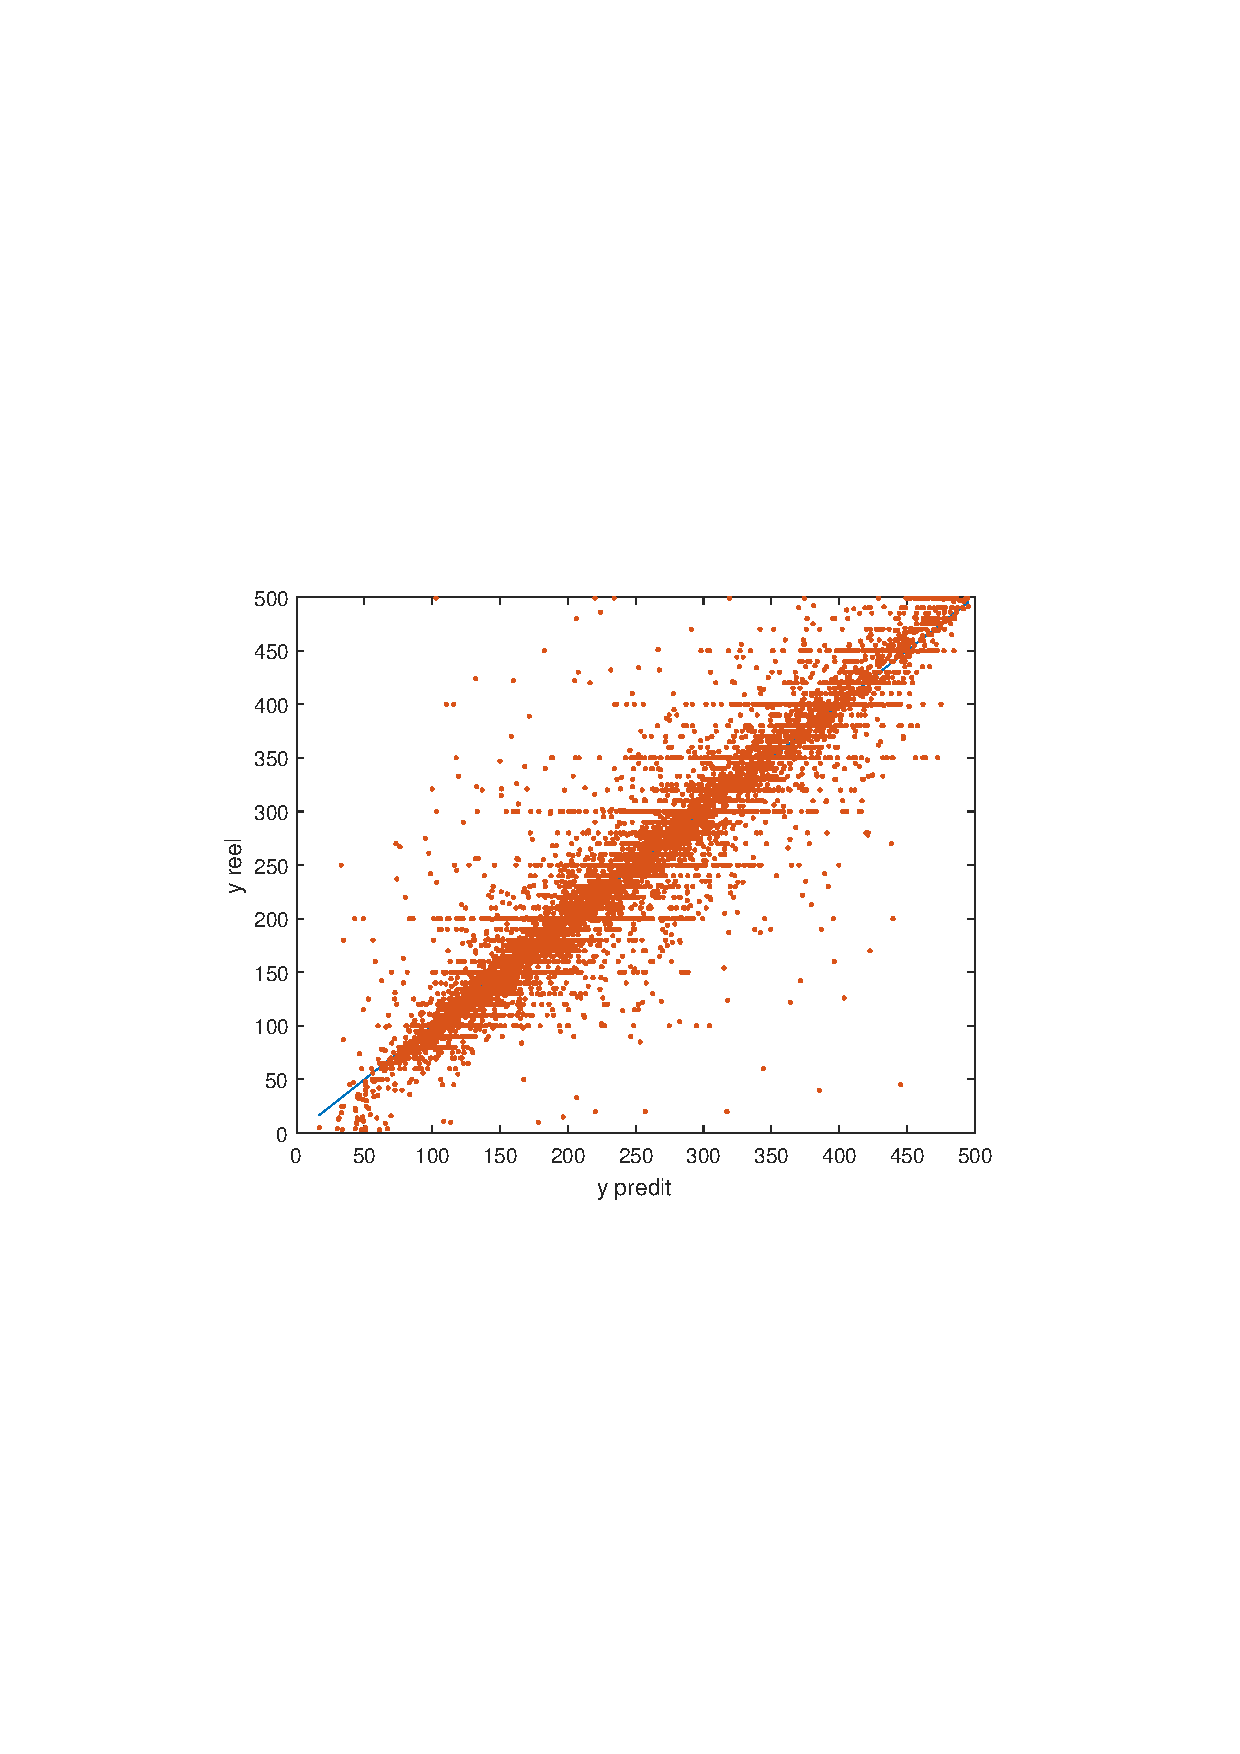
\includegraphics[trim = 3cm 9cm 3cm 9cm, clip]{yreelypredit.pdf}
\captionof{figure}{$y_{reel}(3)$ en fonction de $y_{predit}(3)$}
\label{fig1}
\end{center}

\begin{multicols}{2}

\section{Etude des erreurs}

Intéressons-nous maintenant aux erreurs. Plaçons-nous dans un premier temps dans le cadre du counting game. Nous avons représenté l'écart entre$ y_{reel}(3)$ et $y_{predit}(3)$ en fonction de $ y_{reel}(3)$, ce qui nous donne la figure \ref{fig2}.\\

\end{multicols}

\begin{center}
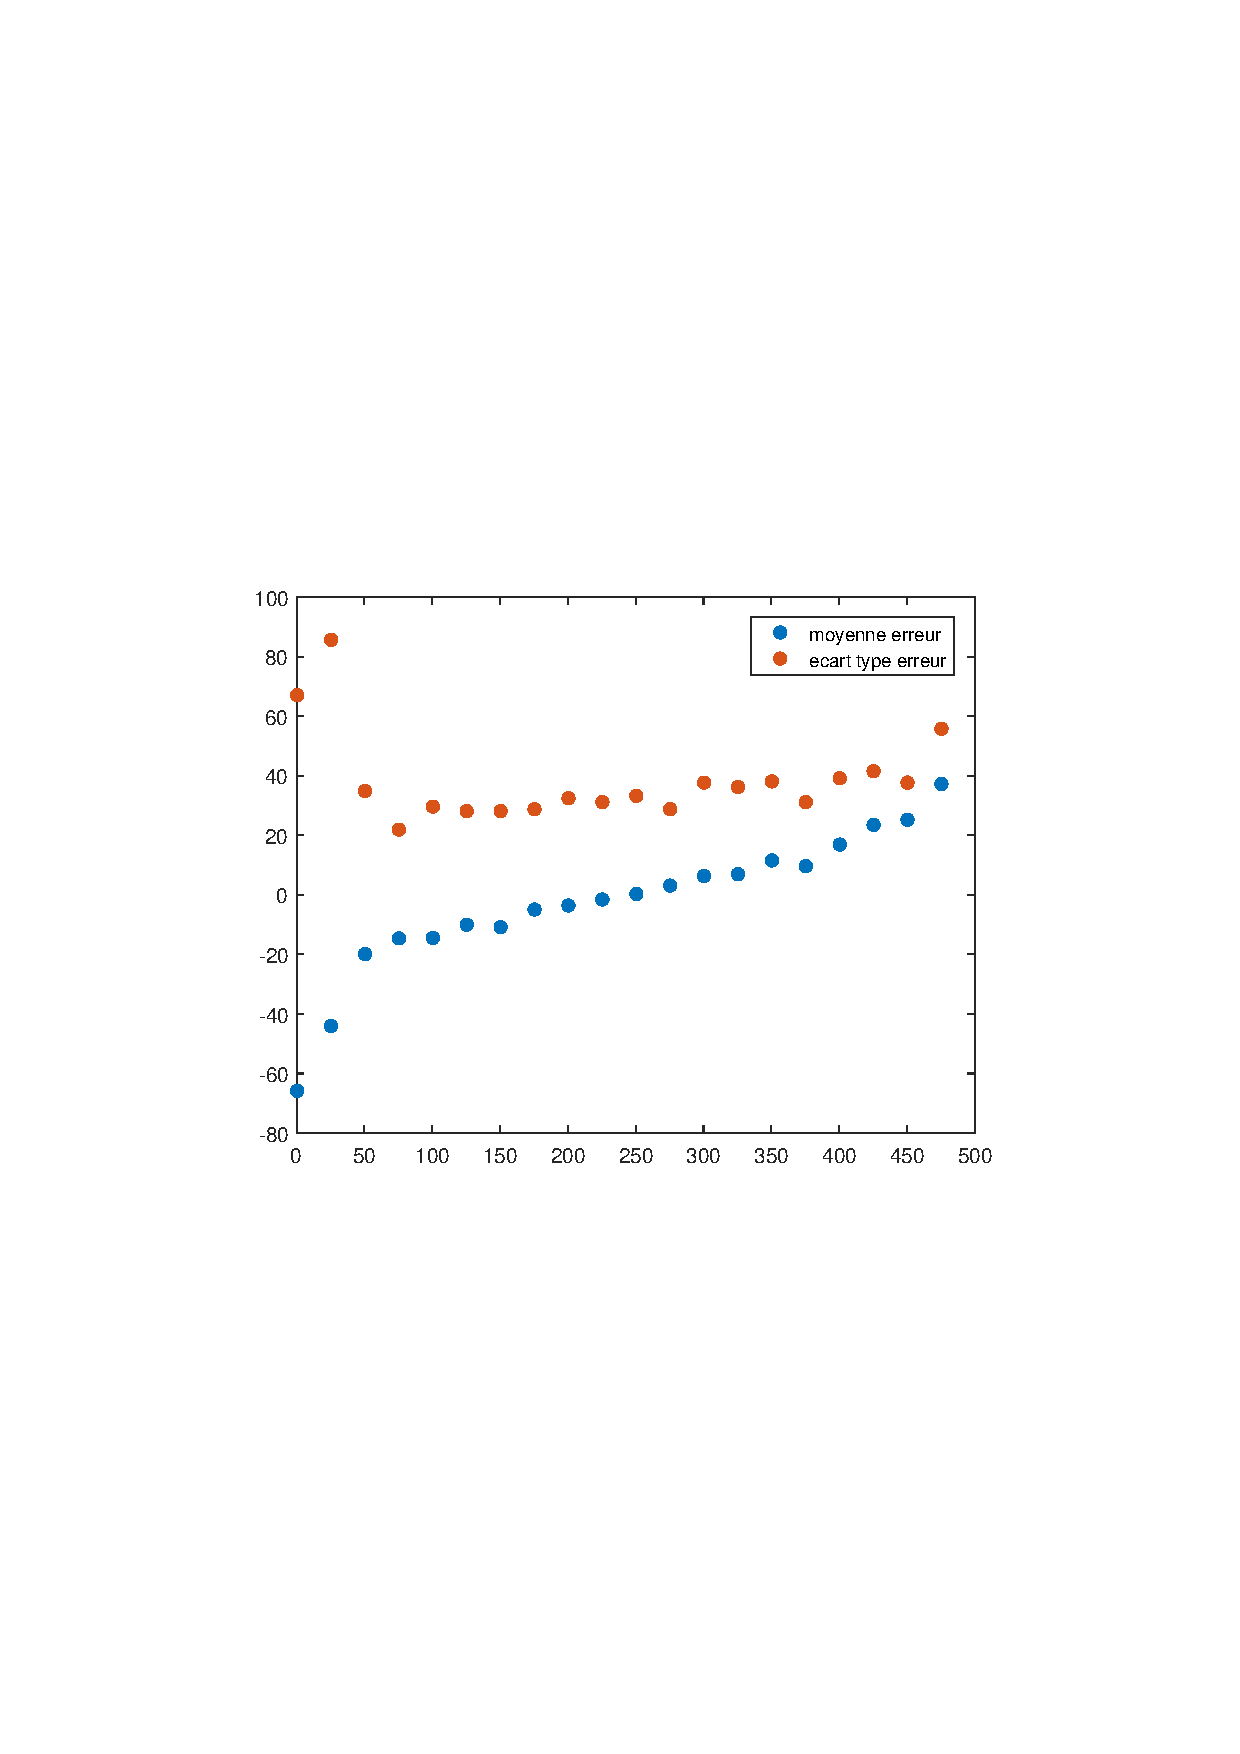
\includegraphics[trim = 3cm 9cm 3cm 9cm, clip]{residu.pdf}
\captionof{figure}{Résidu}
\label{fig2}
\end{center}

\begin{multicols}{2}

La figure \ref{fig3} présente l'écart-type et la moyenne de ces erreurs. Nous pouvons constater que l'écart type est constant tant que les valeurs de $y_{reel}(3)$ ne sont ni trop faible (inférieures à 50), ni trop élevées (supérieures à 450). Il ne nous est donc pas complètement possible de valider l'homocédasticité des erreurs. Ceci peux venir du manque de résultats dans les intervalles [0; 50] et [450; 500]. Il faut aussi prendre en compte que les résultats de l'expérience étaient bornés. Nous obtenons des résultats similaires en utilisant la seconde série de données (gauging game).\\

\end{multicols}

\begin{center}
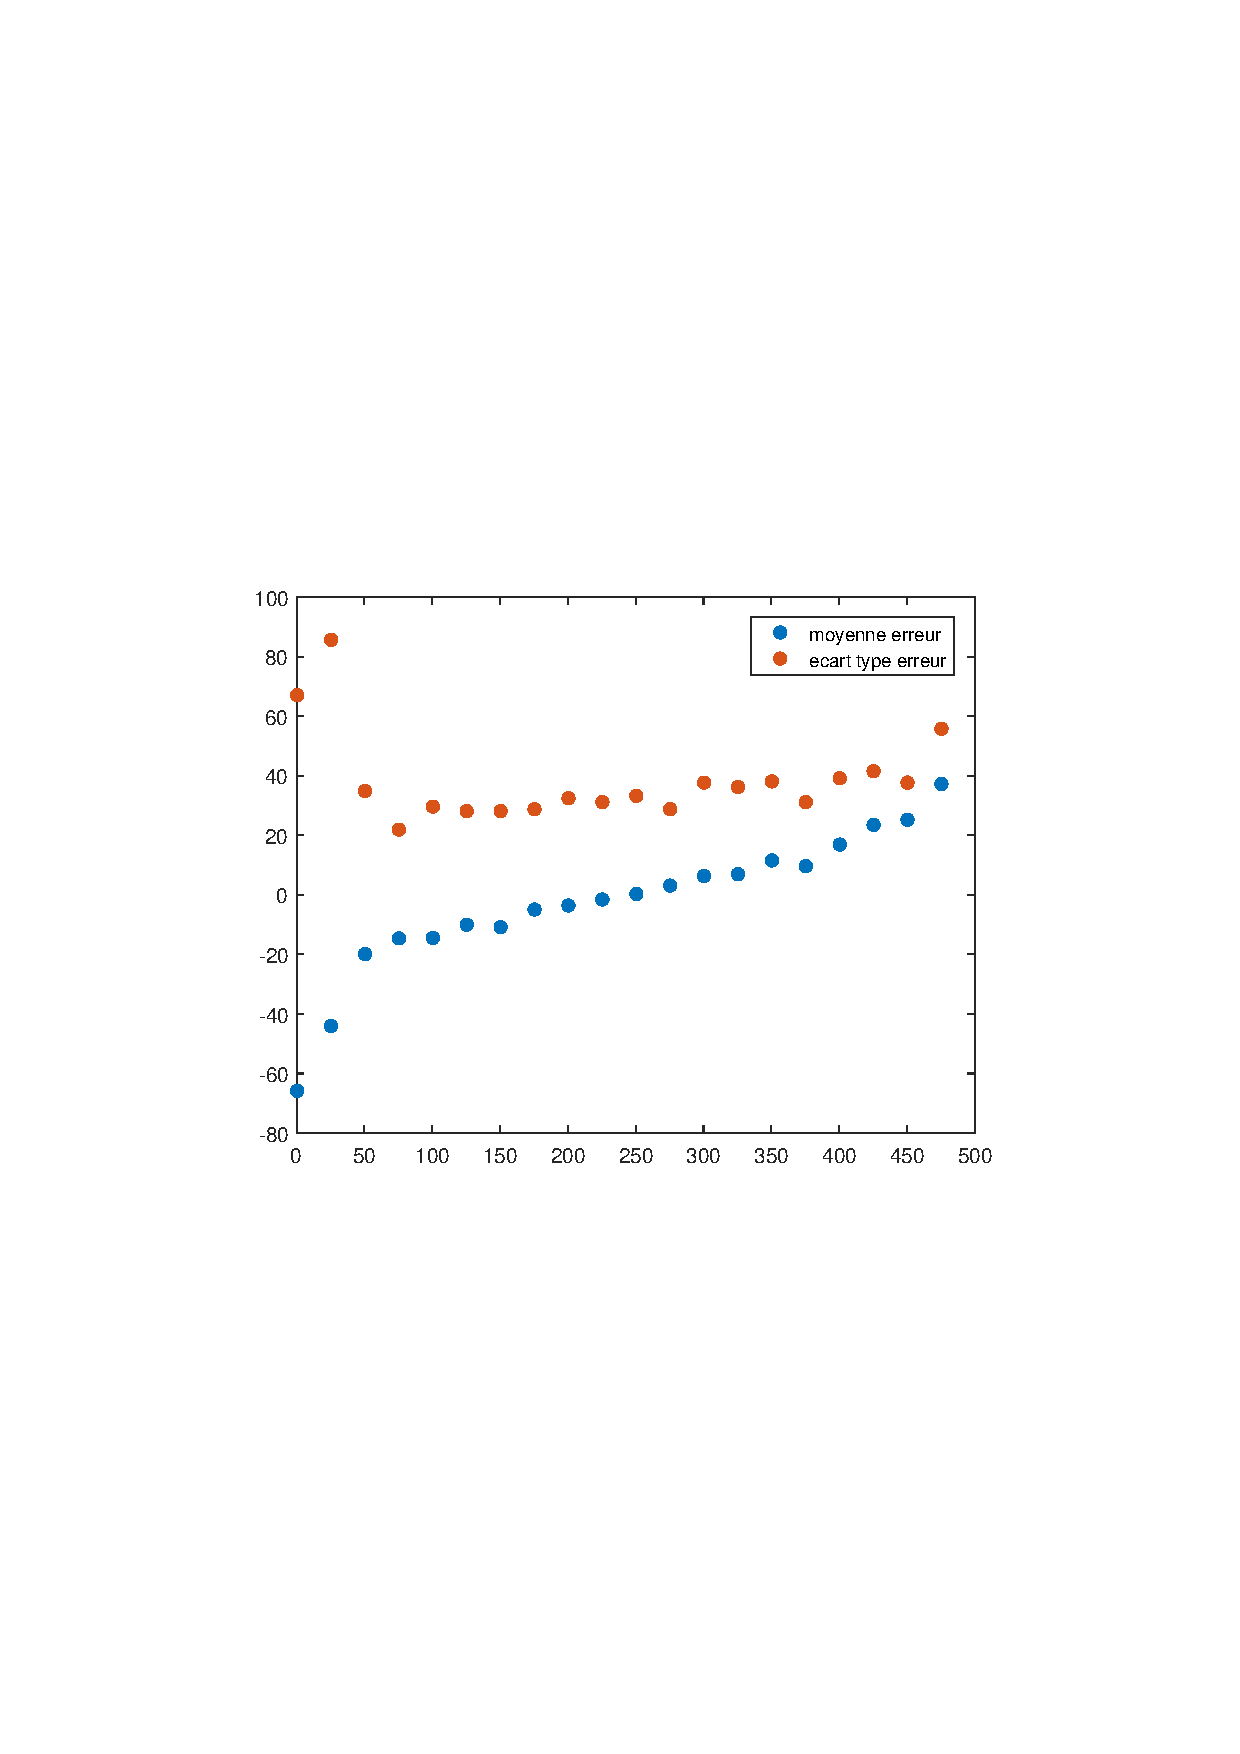
\includegraphics[trim = 3cm 9cm 3cm 9cm, clip]{residuMoyen.pdf}
\captionof{figure}{Moyenne et écart-type des résidus}
\label{fig3}
\end{center}

\begin{multicols}{2}

\section{Bootstrap}

Nous allons maintenant vérifier si le coefficient $\gamma$ devant l'opinion initiale est significatif. Pour cela, suite au bootstrap, nous avons obtenus l'histogramme présent en figure \ref{fig4} (obtenu avec la série counting game). Il nous est alors possible d'encadrer à 95\% la valeur de $\gamma$. Ces valeurs sont résumées dans la table 3.2. Ainsi, on peut affirmer, à 95\%, que $\gamma$ est non nul. L'opinion initiale joue donc bien un rôle dans la décision finale.

\end{multicols}

\begin{center}
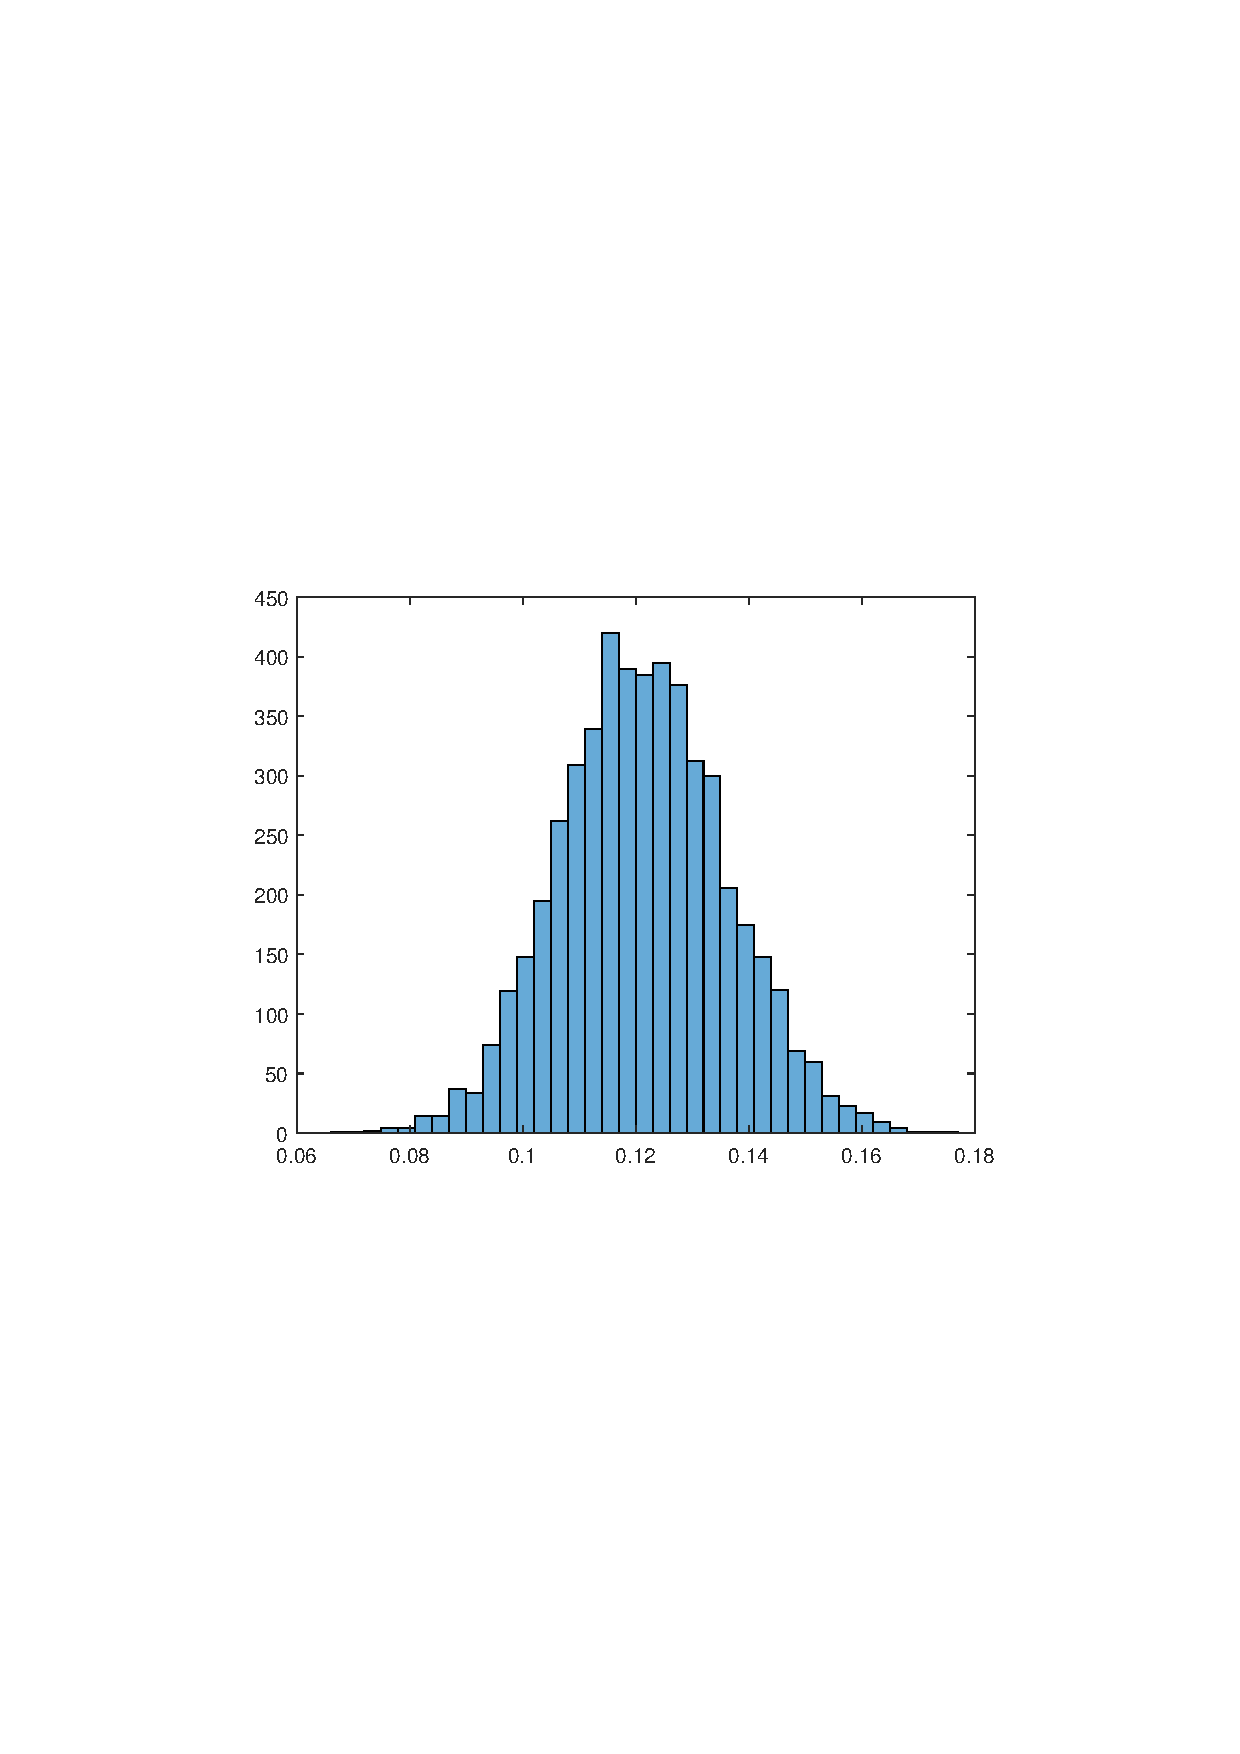
\includegraphics[trim = 3cm 9cm 3cm 9cm, clip]{bootstrap.pdf}
\captionof{figure}{Répartition des différentes valeurs de $\gamma$}
\label{fig4}
\end{center}

\begin{table}
	\begin{tabular}{|p{4cm}|p{4.5cm}|p{4.5cm}|}
		\hline
 & Borne inférieure & Borne supérieure  \tabularnewline
		\hline
Gauging game & 0.0531 &  0.1236  \tabularnewline
		\hline
Counting game & 0.0937 & 0.1510 \tabularnewline
		\hline
	\end{tabular}
	\caption{Encadrement à 95\% de $\gamma$}
\end{table}

\bibliographystyle{plain}
\bibliography{references}






\end{document}
